%
% keys.tex -- slide template
%
% (c) 2021 Prof Dr Andreas Müller, OST Ostschweizer Fachhochschule
%
\bgroup
\begin{frame}[t]
\setlength{\abovedisplayskip}{5pt}
\setlength{\belowdisplayskip}{5pt}
\frametitle{Schlüsselerzeugung}
\vspace{-20pt}
\begin{columns}[t,onlytextwidth]
\begin{column}{0.48\textwidth}
\begin{center}
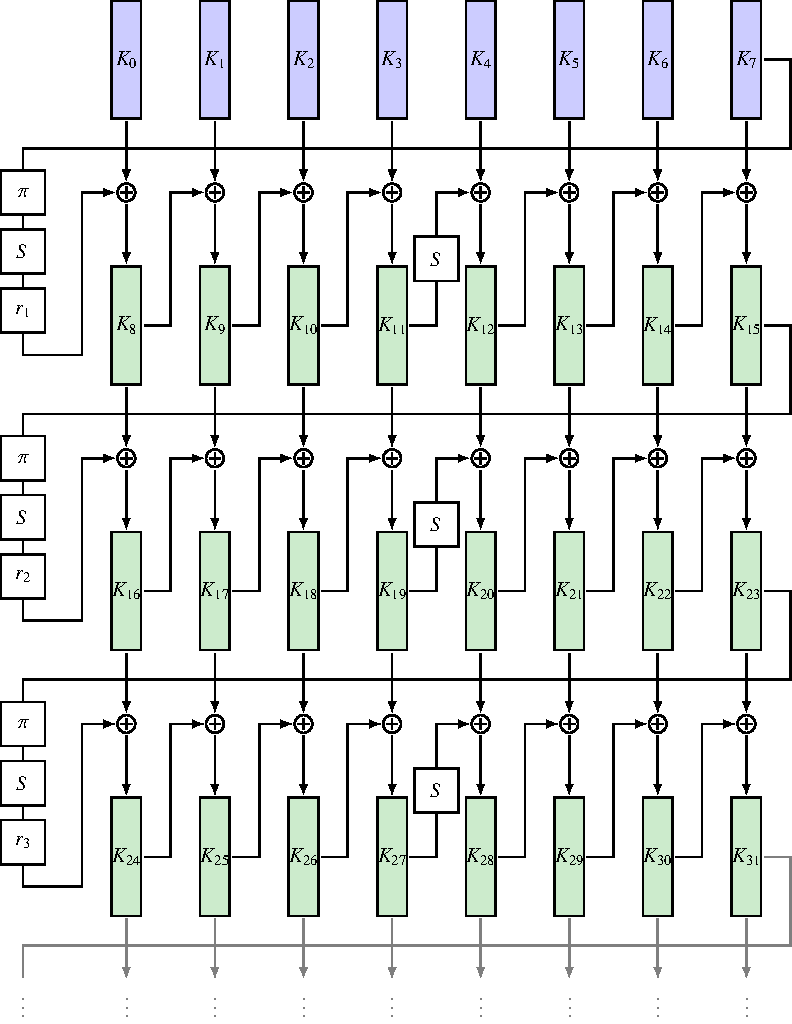
\includegraphics[width=\textwidth]{../../buch/chapters/90-crypto/images/keys.pdf}
\end{center}
\end{column}
\begin{column}{0.48\textwidth}
\begin{block}{Algorithmus}
\begin{enumerate}
\item<2->
Startblock: begebener Schlüssel
\item<3->
Zeilenpermutation:
$\pi=\mathstrut$ Multiplikation mit $Z^3=Z^{-1}$
\item<4-> $S$-Box
\item<5-> $r_i$: Addition einer Konstanten
\[
r_i = (\texttt{02}_{16})^{i-1}
\]
\end{enumerate}
\end{block}
\end{column}
\end{columns}
\end{frame}
\egroup
